\section{Digital Electronics and Operating Systems}

\begin{frame}
  \frametitle{Digital Electronics and Operating Systems}
  
  \begin{itemize}
      \item Electronics: Analog and Digital
      \item Enter the Sandman: Microcontroller
      \item Productivity Nightmares: Primary Solutions
      \item Open Source OSes
      \item Linux and Free Software
  \end{itemize}
  
    \centering
  
\includegraphics[width=2.5cm]{tux_dig}  
  
\end{frame}


\begin{frame}{Electronics: Analog and Digital}

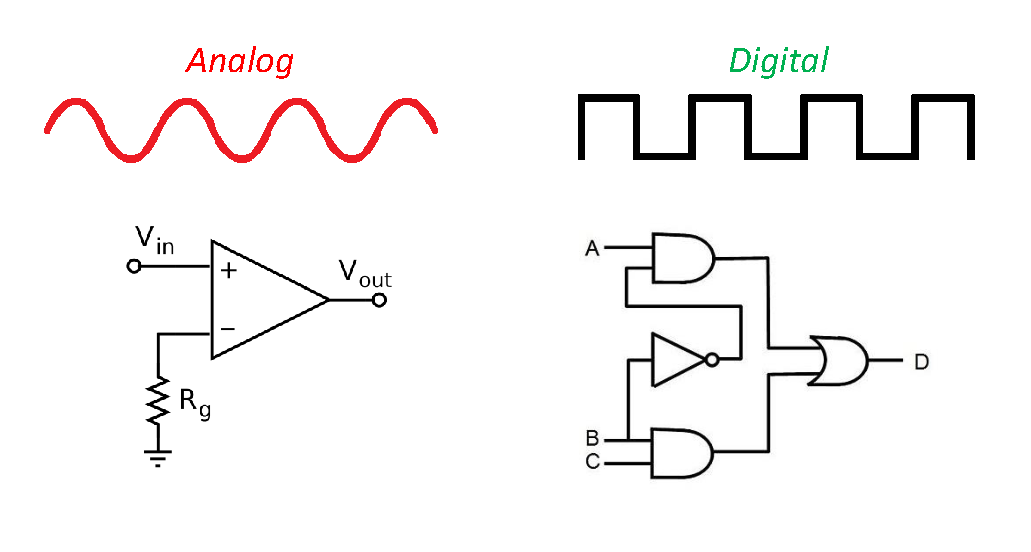
\includegraphics[width=10cm]{AD}

\end{frame}


\begin{frame}{Enter the Sandman: Microcontroller}

\begin{itemize}
    \item 
Gate + Clock $\Rightarrow$ Microprocessor
    \item 
Microprocessor + Peripherals $\Rightarrow$ Microcontroller
    \item 
Microcontroller + CoProcessors $\Rightarrow$ Embedded Processor
\end{itemize}

    \centering
  
\includegraphics[width=2.5cm]{tux_sandman}

\end{frame}


\begin{frame}{Productivity Nightmares: Primary Solutions}
    Serious Challenges:
    \begin{itemize}
        \item Managing Peripherals 
        \item Moore's Law
        \item Programming APIs
        \item Hardware Dependency
    \end{itemize}
    
    Recommended Solutions:
    \begin{itemize}
        \item Open Hardware
            \begin{itemize}
                \item Arduino/Genuino
            \end{itemize}
        \item Open Source Hardware Programming Platforms
        \begin{itemize}
             \item Mbed
        \end{itemize}
        \item Operating System
    \end{itemize}
\end{frame}



\begin{frame}{Open Source OSes}
    
    \begin{itemize}
  
  \item \textbf{FreeRTOS}
  \item \textbf{RIOT}
  \item Contiki
  \item TinyOS
  \item OpenWSN
  \item Zephyr
  \item \textbf{GNU/Linux}
  
    \end{itemize}
    
\end{frame}


\begin{frame}{Linux and Free Software}

Advantages of Linux and Free Software for embedded systems:

\begin{itemize}
    \item Re-using components
    \item Low cost
    \item Full control
    \item Quality
    \item Easy testing of new features
    \item Community support
\end{itemize}
    
\end{frame}



\begin{frame}{Re-using components}
    \begin{itemize}
        \item  The key advantage of Linux and open-source in embedded
systems is the \textbf{ability to re-use components}
\item The open-source ecosystem \textbf{already provides} many
components for standard features, from hardware support to
network protocols, going through multimedia, graphic,
cryptographic libraries, etc.
\item As soon as a hardware device, or a protocol, or a feature is
wide-spread enough, high chance of having open-source
components that support it.
\item Allows to \textbf{quickly design and develop} complicated products,
\textbf{based on existing components}.
\item No-one should re-develop yet another operating system kernel,
TCP/IP stack, USB stack or another graphical toolkit library.
\item Allows to \textbf{focus on the added value of your product}.
    \end{itemize}    
\end{frame}


\begin{frame}{Low cost}
    \begin{itemize}
        \item Free software \textbf{can be duplicated} on as many devices as you
want, \textbf{free of charge}.
\item If your embedded system uses only free software, you can
reduce the \textbf{cost of software licenses to zero}. Even the
development tools are free, unless you choose a commercial
embedded Linux edition.
\item Allows to have a higher budget for the hardware or to
increase the company’s skills and knowledge
    \end{itemize}    
\end{frame}


\begin{frame}{Full control}
    \begin{itemize}
        \item With open-source, you have the source code for all
components in your system
\item Allows \textbf{unlimited modifications, changes, tuning, debugging,
optimization}, for an unlimited period of time
\item Without lock-in or dependency from a third-party vendor
\item To be true, non open-source components must be avoided
when the system is designed and developed
\item Allows to have \textbf{full control over the software part} of your
system
    \end{itemize}    
\end{frame}


\begin{frame}{Quality}
    \begin{itemize}
        \item Many open-source components are \textbf{widely used}, on millions of
systems
\item Usually \textbf{higher quality} than what an in-house development can
produce, or even proprietary vendors
\item Of course, not all open-source components are of good
quality, but most of the widely-used ones are.
\item Allows to \textbf{design your system with high-quality
components} at the foundations
    \end{itemize}    
\end{frame}


\begin{frame}{Easy testing of new features}
    \begin{itemize}
        \item Open-source being freely available, it is \textbf{easy to get a piece of
software and evaluate it}
\item Allows to \textbf{easily study several options} while making a choice
\item Much \textbf{easier than purchasing} and demonstration procedures
needed with most proprietary products
\item Allows to \textbf{easily explore new possibilities} and solutions
    \end{itemize}    
\end{frame}


\begin{frame}{Community support}
    \begin{itemize}
        \item Open-source software components are developed by
communities of developers and users
\item This community can provide a \textbf{high-quality support}: you can
directly contact the main developers of the component you
are using. The likelyhood of getting an answer doesn't depend
what company you work for.
\item Often better than traditional support, but one needs to
understand how the community works to properly use the
community support possibilities
\item Allows to \textbf{speed up the resolution of problems} when
developing your system
    \end{itemize}    
\end{frame}


\begin{frame}{Linux Disadvantages!!!}

\begin{itemize}
    \item
     Linux certainly is a robust and developer-friendly OS
     \item Linux will have many uses in embedded devices, particularly
ones that provide graphically rich user interfaces.
\item
Linux has a disadvantage when compared to other embedded operating systems:
\begin{itemize}
\item Memory footprint
\item It simply will not run on 8 or 16-bit MCUs
\item Real-time operations problem
\end{itemize}
\end{itemize}


        \centering
  
\includegraphics[width=3cm]{tux_weak}


\end{frame}